% !TeX spellcheck = en_US
\documentclass[aspectratio=1610]{beamer}
\mode<presentation>
{
  \usetheme{Boadilla}
  \setbeamercovered{transparent}
  
  \definecolor{cobalt}{rgb}{0.0, 0.20, 0.50}
  
  \usecolortheme[named=cobalt]{structure}
  %\usecolortheme{lily}
  %\setbeamercolor{headline}{fg=cyan!80!black}
  % \setbeamercolor{frametitle}{bg=white}.
}

\makeatletter
\define@key{beamerframe}{wide}[10pt]{%
	\def\beamer@cramped{\itemsep #1\topsep0.5pt\relax}}
\makeatother
	

\usepackage[english]{babel}
\usepackage[utf8]{inputenc}
\usepackage{times}
\usepackage[T1]{fontenc}
\usepackage{array}
\usepackage{xcolor}
\usepackage{colortbl}
\usepackage{booktabs}

\title[Winter - Lecture 4] % (optional, use only with long paper titles)
{Macroeconomic Theory and Policy: Lecture  W4 (Ch.11)}

\author[University of Toronto] % (optional, use only with lots of authors)
{}
\date[] % (optional, should be abbreviation of conference name)

\begin{document}

\begin{frame}
  \titlepage
\end{frame}

\begin{frame}[wide]{What are You Going to Learn (Ch. 11)}
	\begin{itemize}
		\item The IS curve
		\begin{itemize}
			\item The foundation component of the short-run model
			\item Illustrates the negative correlation between the real interest rate and short-run output
		\end{itemize}
		\item Understanding how shocks to consumption, investment, government purchases, or net exports—referred to as "aggregate demand shocks" -- can alter the position of the IS curve
		\item Highlighting investment as the primary channel through which fluctuations in real interest rates impact GDP in the short run
		\item The life-cycle/permanent-income hypothesis can form the microfoundations for the IS curve
	
		
	\end{itemize}
\end{frame}

\begin{frame}[wide]{Introduction to the IS Curve}
	\begin{itemize}
%		\item The central bank can influences the level of economic activity in the short run by
%		\begin{itemize}
%			\item targets the overnight lending rate, which is highly correlated with the short-term nominal interest rate at which people borrow and lend in financial markets
%		\end{itemize}
		\item The basic story is as follows: 
		\[\uparrow \text{Interest Rate} \implies \downarrow \text{Investment} \implies \downarrow \text{Output}\]
		\begin{itemize}
			\item The same story can apply to college students, individuals taking out loans, financial advisors, firms and even people does not borrow money
		\end{itemize}
		\vspace{8mm}
		\item The IS curve illustrates the negative relationship between interest rates and short-run output		
	\end{itemize}
\end{frame}

\begin{frame}[wide]{Introduction to the IS Curve}
	\begin{itemize}
		\item IS curve captures how a high interest rate reduces output in the short run (and vice versa) through which this occurs is investment
	\end{itemize}
	\begin{figure}
		\centering
		\includegraphics[width=0.45\linewidth]{"Figures/fig 11_01"}
	\end{figure}
	
\end{frame}

\begin{frame}[wide]{Setting Up the Economy}
	\begin{itemize}
		\item The short-run model, just like the long-run model of economic growth, is based on a simple economy and various assumptions
		\item First, define how resource are spent in an economy
		\item The national income accounting identity
		\begin{itemize}
			\item total resources available to the economy equal total uses
		\end{itemize}
		\[Y_t = C_t + I_t + G_t +EX_t -IM_t\]
		\item[] where
		\begin{itemize}
			\item[] $C_t$ is the consumption
			\item[] $Y_t$ is the output
			\item[] $I_t$ is the investment
			\item[] $G_t$ is the government spending
			\item[] $EX_t-IM_t$ is the net export
		\end{itemize}
	\end{itemize}
\end{frame}

\begin{frame}[wide]{Setting Up the Economy}
	Five additional equations to solve the model
	\[C_t = \bar{a_c}\bar{Y}_t	\]
	\[G_t = \bar{a_g}\bar{Y}_t	\]
	\[EX_t = \bar{a_{ex}}\bar{Y}_t	\]
	\[IM_t = \bar{a_{im}}\bar{Y}_t	\]
	\[\frac{I_t}{\bar{Y}_t} = \bar{a}_i - \bar{b}\left(R_t -\bar{r}\right)\]
	\begin{itemize}
		\item Except for investment, all component are a proportion of the potential output $\bar{Y}_t$
		\item Investment is determined by an exogenous part and is depends on fluctuations in the interest rate from its long-run level, $\bar{r}$
	\end{itemize}
\end{frame}

\begin{frame}[wide]{Consumption, Government Purchases, Net Export}
	\begin{itemize}
		\item Empirically $\bar{a}_c$ in the consumption equation estimated to be approximately 2/3
		\vspace{2mm}
		\begin{itemize}
			\item two out of every three dollars of GDP is attributed to consumption
			\item as suggested by the permanent income hypothesis, the share is relatively stable
		\end{itemize}
		\vspace{8mm}
		\item Furthermore, we set government purchases, exports, and imports are all assumed to be long-run fractions of output as see in the data
		\vspace{2mm}
		\begin{itemize}
			\item The other variables can change very often, but for simplicity, we will assume them to be constant for now
		\end{itemize}
	\end{itemize}
\end{frame}

\begin{frame}[wide]{The Investment Equation}
	\[\frac{I_t}{\bar{Y}_t} = \bar{a}_i - \bar{b}\left(R_t -\bar{r}\right)\]
	\vspace{4mm}
	\begin{itemize}
		\item Part of investment is determined by a constant fraction $\bar{a}_i$ of potential output, $\bar{Y}$
		\vspace{3mm}
		\item The amount of investment also depends on the gap between the real interest rate $R_t$ and the marginal product of capital ($\bar{r}$)
		\vspace{2mm}
		\begin{itemize}
			\item The effect of the difference would be depend on the parameter $\bar{b}$
		\end{itemize}
		\vspace{3mm}
		\item The long-run interest rate can be interpret as the Marginal Product of Capital (MPK) 
	
	\end{itemize}
\end{frame}

\begin{frame}[wide]{Marginal Product of Capital (MPK)}
	\begin{itemize}
		\item MPK: Amount of additional output the firm can produce by investing in one more unit of capital
		\vspace{4mm}
		\item Here, the MPK is determined in the long-run model, which is exogenous and time invariant in this short-run model 
		
	\end{itemize}
\end{frame}

\begin{frame}[wide]{Marginal Product of Capital (MPK)}
	\begin{itemize}
		\item In the short run, the gap between MPK and the real interest rate determine investment
		\vspace{1mm}
		\begin{itemize}
			\item If $R_t > MPK$, firm/capital owner is better off to invest in financial market (saving), investment falls
			\item If $R_t < MPK$, firm/capital owner is better off to invest in firm (or renting capital), investment rises
			\item In the long run, all these adjustment would be made and thus $R_t = \bar{r} = MPK$
		\end{itemize}
		\vspace{4mm}
		\item Why would $R_t$ be different from in $\bar{r}$
		\begin{itemize}
			\item Capital takes time to build, Central bank's policy, etc
		\end{itemize}
	\end{itemize}
\end{frame}

\begin{frame}[wide]{Potential Output}
	\begin{itemize}
		\item In the long run, $R_t - \bar{r}$, the investment is then
		\[I_t = \bar{a}_i \bar{Y}\]
		\vspace{1mm}
		\item Summing all the equations, we have 
		\[Y_t = C_t+G_t+EX_t-IM_t +I =\bar{a}_c \bar{Y} +\bar{a}_g \bar{Y} + \bar{a}_{ex} \bar{Y} - \bar{a}_{im} \bar{Y} + \bar{a}_i \bar{Y}\]
		\[\quad = \left(\bar{a}_c  +\bar{a}_g  + \bar{a}_{ex} - \bar{a}_{im} + \bar{a}_i\right) \bar{Y}\]
		\vspace{1mm}
		\item Then, together with $\left(\bar{a}_c  +\bar{a}_g  + \bar{a}_{ex} - \bar{a}_{im} + \bar{a}_i\right) = 1$ implies the economy is in the long run, which $Y_t = \bar{Y}$
		\vspace{1mm}
		\item This would also imply that the only source causing the output be deviate from $\bar{Y}$ is $R_t - \bar{r}$ and/or when $\left(\bar{a}_c  +\bar{a}_g  + \bar{a}_{ex} - \bar{a}_{im} + \bar{a}_i\right) \neq 1$ in this simple model
	\end{itemize}
\end{frame}

\begin{frame}[wide]{The Setup of the Economy for the IS Curve}
	\[C_t = \bar{a_c}\bar{Y}_t	\]
	\[G_t = \bar{a_g}\bar{Y}_t	\]
	\[EX_t = \bar{a_{ex}}\bar{Y}_t	\]
	\[IM_t = \bar{a_{im}}\bar{Y}_t	\]
	\[\frac{I_t}{\bar{Y}_t} = \bar{a}_i - \bar{b}\left(R_t -\bar{r}\right)\]
	\[Y_t = C_t + I_t + G_t +EX_t -IM_t\]
	\begin{itemize}
		\item Six equations
		\item Endogenous variables: $Y_t$, $C_t$, $I_t$, $G_t$, $EX_t$, $IM_t$
		\item Exogenous variables/parameters: $\bar{Y}$, $\bar{r}$, $\bar{a}_c$, $\bar{a}_g$, $\bar{a}_{ex}$, $\bar{a}_{im}$, $\bar{a}_i$, $\bar{b}$, $R_t$
	\end{itemize}
\end{frame}

\begin{frame}[wide]{Deriving the IS Curve}
	\begin{itemize}
		\item Recall the definition of short-run output
		\[\tilde{Y}_t = \frac{Y_t - \bar{Y}}{\bar{Y}} = \frac{Y_t}{\bar{Y}} -1\]
		\vspace{4mm}
		\item Sub in $Y_t= \left(\bar{a}_c  +\bar{a}_g  + \bar{a}_{ex} - \bar{a}_{im} + \bar{a}_i -\bar{b} (R_t - \bar{r})\right) \bar{Y}$
		\[\frac{Y_t}{\bar{Y}} -1 = \bar{a}_c  +\bar{a}_g  + \bar{a}_{ex} - \bar{a}_{im} + \bar{a}_i -\bar{b} (R_t - \bar{r}) - 1\]
		\vspace{4mm}
		\item Let $\bar{a} = \bar{a}_c  +\bar{a}_g  + \bar{a}_{ex} - \bar{a}_{im} + \bar{a}_i -1$,
		\[\tilde{Y}_t = \frac{Y_t}{\bar{Y}} -1 =  \bar{a}-\bar{b} (R_t - \bar{r})\]
	\end{itemize}
\end{frame}

\begin{frame}[wide]{Deriving the IS Curve}
	\begin{itemize}
		\item Variable $C$, $G$, $XM$ and $IM$ can be deviated from their long-run level in the short run, 
		\[\bar{a} = \bar{a}_c  +\bar{a}_g  + \bar{a}_{ex} - \bar{a}_{im} + \bar{a}_i - 1 \neq 0\]
		\begin{itemize}
			\item It can be interpret as aggregate demand shock
		\end{itemize}
		\vspace{3mm}
		\item Rewrite the formula above 
		\[\tilde{Y} = \bar{a} - \bar{b} (R_t - \bar{r})\]
		\vspace{3mm}
		\item In the long run, $\tilde{Y} = 0$ and $\bar{a} = 0$
		\[R_t = \bar{r}\]
	\end{itemize}
\end{frame}

\begin{frame}[wide]{Why Is It Called the "IS Curve"?}
	\begin{itemize}
		\item The concept was introduced by John R. Hicks
		\item "IS" stands for "investment equals savings."
		\[Y= C+I+G+EX-IM\]
		\[Y-C-G + (IM-EX) = I\]
		\item Add and subtract T, government tax
		\[(Y-T-C)+(T-G) + (IM-EX) = I\]
		\begin{itemize}
			\item $Y-T-C$ is private saving
			\item $T-G$ is the public saving 
			\item $IM-EX$ is foreign saving
		\end{itemize}
	\end{itemize}
\end{frame}

\begin{frame}[wide]{Using the IS Curve}
	\[\tilde{Y} = \bar{a} - \bar{b} (R_t - \bar{r}) \implies R_t = \bar{r} + \frac{\bar{a}}{\bar{b}}  -\frac{\tilde{Y}}{\bar{b}}\]
	In the long run, $\bar{a}=0$, $\tilde{Y} = 0$
	\begin{figure}
		\centering
		\includegraphics[width=0.45\linewidth]{"Figures/fig 11_02"}
	\end{figure}
	
\end{frame}

\begin{frame}[wide]{A Change in the Interest Rate}
	\begin{itemize}
		\item A change in the real interest rate moves the economy along the IS curve
		\vspace{6mm}
		\begin{enumerate}
			\item Increase in interest rate (exogenous)
			\item Increase in borrowing costs/opportunity cost of investing
			\item Decrease in demand for investment
			\item Decrease in output ($Y_t$)
			\item Move up along the IS curve
		\end{enumerate}
	\end{itemize}
	
\end{frame}

\begin{frame}[wide]{An Increase in the Real Interest Rate to R'}
	\begin{itemize}
		\item An increase to R’ in the real interest rate is a movement along the IS curve that moves the economy from A to B, resulting in a decline in output in the short run
	\end{itemize}
	\begin{figure}
		\centering
		\includegraphics[width=0.5\linewidth]{"Figures/fig 11_03"}
	\end{figure}
	
\end{frame}

\begin{frame}[wide]{A Change in the Interest Rate}
	\begin{itemize}
		\item How much would the output change as the interest rate increase? 
		\begin{itemize}
			\item It depends on $\bar{b}$
		\end{itemize}
		\[R_t = \frac{\bar{a}}{\bar{b}} +\bar{r} - \frac{1}{\bar{b}} \tilde{Y} \]
		\vspace{3mm}
		\item The IS curve would be flatter as the slope $\left(\frac{1}{\bar{b}}\right)$ decreases
		\vspace{3mm}
		\item The same change in the interest rate would be associated with larger changes in output
	\end{itemize}
\end{frame}

\begin{frame}[wide]{An Aggregate Demand Shock}
	\begin{itemize}
		\item Suppose that there information technology boom create an investment boom
		\vspace{4mm}
		\begin{enumerate}
			\item Increase in optimism
			\item Increase demand for capital
			\item Increase in $\bar{a}_i$, which increase $\bar{a}$
			\item Increase investment at a given interest rate $R_t$
			\item IS curve shift to the right
		\end{enumerate}
	\end{itemize}
\end{frame}

\begin{frame}[wide]{An Aggregate Demand Shock}
	\begin{itemize}
		\item The effect of a positive aggregate demand shock that raises $\bar{a}$ from 0 to $\bar{a}'$
		\item IS curve shifts out, moving the economy from point A to point B
		\begin{itemize}
			\item Holding $R=\bar{r}$, the output $\tilde{Y}$ move from 0 to $\bar{a}'$
		\end{itemize}
		\item Aggregate demand shocks typically result in one-for-one changes in short-run output
	\end{itemize}
	\begin{figure}
		\centering
		\includegraphics[width=0.4\linewidth]{"Figures/fig 11_04"}
	\end{figure}
	
\end{frame}

\begin{frame}[wide]{A Shock to Potential Output}
	\begin{itemize}
		\item Suppose there is a discovery of a new technology (one possibility)
		\begin{enumerate}
			\item Increase in potential output
			\item Increase in actual output
			\item Short-run output unchanged
		\end{enumerate}
		\vspace{4mm}
		\item Recall $\tilde{Y} = \frac{Y_t}{\bar{Y}_t} - 1$. If the economy start from long-run equilibrium, if $Y_t$ and $\bar{Y}_t$ increase by the same amount, the ratio $Y_t/\bar{Y}_t$ will equal to 1 and $\tilde{Y} = 0$
		\vspace{3mm}
		\item Some shock to potential output may change other parameters
		\vspace{2mm}
		\begin{itemize}
			\item For example, an earthquake will reduce actual and potential output by the same amount and also may change the MPK as capital stock was destroyed
		\end{itemize}
	\end{itemize}
\end{frame}

\begin{frame}[wide]{Microfoundations of the IS Curve}
	\begin{itemize}
		\item Microfoundations:	Explain the microeconomic behavior that establishes the demands for $C$, $I$, $G$, $EX$ and $IM$
		\vspace{3mm}
		\item In modern Macroeconomics, Microfoundations serves as the fundamental building blocks for macroeconomic models, ensuring that aggregate economic phenomena are derived from individual-level decisions
		\vspace{3mm}
		\item That is because aggregating individual behaviors to derive macroeconomic variables, ensuring that the macro-level outcomes are consistent with micro-level actions
		\vspace{3mm}
		\item Macro-economist model consumption and investment of the aggregate economy much like in the consumption model and investment model (in ch. 16/17)
		
	\end{itemize}
\end{frame}

\begin{frame}[wide]{Microfoundations of the IS Curve}
	\begin{itemize}
		\item There are often individual deviations from the aggregate macroeconomic behavior. However, when we aggregate, the outliers tend to average out
		\vspace{4mm}
		\begin{itemize}
			\item For instance, a particular individual may spend all (or most) of his or her income on basketball tickets
			\vspace{2mm}
			\item Another individual may spend none (or almost none) of his or her income and save the remainder
			\vspace{2mm}
			\item These idiosyncratic behaviors are not part of our model, and average out when we study the economy as a whole
		\end{itemize}
	\end{itemize}
\end{frame}

\begin{frame}[wide]{Consumption}
	Individuals prefer to smooth their consumption spending over time
	\vspace{3mm}
	\begin{itemize}
		\item Two hypothesis guide how consumption path is modeled: permanent-income hypothesis and life-cycle model
	\vspace{2mm}
		\begin{itemize}
			\item Consumption path is how much an individual consume in each period overtime
		\end{itemize}
		\vspace{2mm}
		\item The life-cycle/permanent-income (LC/PI) hypothesis:
		\vspace{2mm}
		\begin{itemize}
			\item Implies that people smooth their consumption relative to their lifetime income
			\vspace{1mm}
			\begin{itemize}
				\item individuals prefer a small variance in their consumption spending
			\end{itemize}
			\vspace{1mm}
			\item This is why we set consumption proportional to potential output rather than actual output (i.e., $C_t = \bar{a}_c \bar{Y}_t$)
		\end{itemize}
	\end{itemize}
\end{frame}

\begin{frame}[wide]{Consumption}
	\begin{itemize}
		\item Suppose a consumer are given the choice between Option A and Option B
		\vspace{2mm}
		\item Option A:
		\begin{itemize}
			\item Consumption: one piece of cake (\$3) every day Monday through Friday
			\item Income: \$15 on Friday, but you may borrow \$3 a day (at no interest) to consume during the week
		\end{itemize}
		\item Option B:
		\begin{itemize}
			\item Consumption: five pieces of cake (\$15) on Friday
			\item Income: \$15 on Friday
		\end{itemize}
		\vspace{2mm}
		\item The permanent income hypothesis predicts that people will choose Option A
	\end{itemize}
\end{frame}

\begin{frame}[wide]{The Life-Cycle Model of Consumption}
	\begin{itemize}
		\item According to this theory, individuals compensate for this income variation by saving and borrowing in order to consume
		\item People consume more than income, by borrowing or intra-family transfer, start saving as income increase, and dis-save when retire
	\end{itemize}
	\begin{figure}
		\centering
		\includegraphics[width=0.5\linewidth]{"Figures/fig 11_05"}
	\end{figure}
	
\end{frame}

\begin{frame}[wide]{Empirical Evidence (Hsieh, 2003)}
	\begin{itemize}
		\item How do consumers respond to two different types of income shocks in Alaska?
		\vspace{3mm}
		\begin{itemize}
			\item Annual payment from the State of Alaska’s Permanent Fund (from oil revenues)
			\vspace{2mm}
			\begin{itemize}
				\item Large payment relative to income, easy to predict, the amount annouce 6 mths earlier
			\end{itemize}
			\vspace{2mm}
			\item Federal tax refunds
			\vspace{2mm}
			\begin{itemize}
				\item Smaller payment, harder to predict
			\end{itemize}
		\end{itemize}
		\vspace{2mm}
		\item In theory, the LC/PI hypothesis predicts that consumption should not change when the Permanent Fund check or Federal tax refunds are received
	\end{itemize}
\end{frame}

\begin{frame}[wide]{Empirical Evidence}
	\begin{itemize}
		\item Hsieh finds the sample smooth their consumption for the Permanent Fund
		\item But the same is not true in response to a tax refund. For every \$1 of a tax refund, consumers spend 0.30 cents (contradictory to the predictions of the LC/PI hypothesis)
		\item Hsieh interprets this evidence as suggesting that the LC/PI hypothesis works well for large and easy-to-predict changes in income but less well for small and harder-to-predict shocks
	\end{itemize}
\end{frame}

\begin{frame}[wide]{Multiplier Effects}
	\begin{itemize}
		\item Most evidence would suggest that household would not be smoothing consumption perfectly
		\item Let us to augment the consumption equation to include a term that responds to changes in short-run output 
		\begin{itemize}
			\item This yields a multiplier effect
		\end{itemize}
		\item Consumption equal:
		\[\frac{C_t}{\bar{Y}_t} = \bar{a}_c + \bar{x} \tilde{Y}_t\]
		\item[] where $\bar{x}\in (0,1)$ is a parameter that determines how much consumption rises when the economy expands
	\end{itemize}
\end{frame}

\begin{frame}[wide]{Multiplier Effects}
	\begin{itemize}
		\item Solving for the IS curve with this augmented consumption function
		\[Y_t = C_t + I_t + G_t +EX_t -IM_t = \left(\bar{a}_c + \bar{x} \tilde{Y}_t\right)\bar{Y}  + \left(\bar{a}_i - \bar{b}\left(R_t -\bar{r}\right)\right)\bar{Y} + \bar{a}_g \bar{Y}  + \bar{a}_{ex}\bar{Y} - \bar{a}_{im}\bar{Y} \]
		\item Divide it by $\bar{Y}$
		\[\frac{Y_t}{\bar{Y}} =  \bar{a}_c + \bar{x} \tilde{Y}_t  + \bar{a}_i - \bar{b}\left(R_t -\bar{r}\right) + \bar{a}_g   + \bar{a}_{ex} - \bar{a}_{im} \]
		\item Recall that $\bar{a} = \bar{a}_c + \bar{a}_i + \bar{a}_g + \bar{a}_{ex} - \bar{a}_{im} - 1$
		\[\tilde{Y} = \frac{Y_t}{\bar{Y}} -1 =   \bar{x} \tilde{Y}_t   - \bar{b}\left(R_t -\bar{r}\right) + \left(\bar{a}_c + \bar{a}_i + \bar{a}_g   + \bar{a}_{ex} - \bar{a}_{im}  -1 \right)\]
		\[\tilde{Y} = \bar{x} \tilde{Y} +\bar{a} - \bar{b}\left(R_t -\bar{r}\right)\]
	\end{itemize}
\end{frame}

\begin{frame}[wide]{Multiplier Effects}
	\begin{itemize}
		\item Finally, rearrange:
		\[\tilde{Y} = \frac{1}{1-\bar{x}} \times \left(\bar{a} - \bar{b}\left(R_t -\bar{r}\right) \right)\]
		\vspace{2mm}
		\item The second term $\left(\bar{a} - \bar{b}\left(R_t -\bar{r}\right) \right)$ is just the original IS curve
		\vspace{2mm}
		\item The first term $\frac{1}{1-\bar{x}} $ is the multiplier
		\vspace{1mm}
		\begin{itemize}
			\item Given $\bar{x} \in (0,1)$, the multiplier is greater than 1
			\vspace{1mm}
			\item Any changes in the original IS curve (i.e., $\bar{a}$, $\bar{b}$, $R_t$ or $\bar{r}$) would be multiplied
			\vspace{1mm}
			\item Say, $\bar{a}$ increased by 1 percent and $\bar{x} = 0.5$. Given the multiplier $\frac{1}{1-0.5} = 2$, the short run output $\tilde{Y}$ would increase by 2\%
		\end{itemize}
	\end{itemize}
\end{frame}

\begin{frame}[wide]{Multiplier Effects}
	\begin{itemize}
		\item Initial Impact:	Increase in investment leads to job creation among construction workers
		\item Consequent increase in consumption:	New employed would increase their consumption
		\item Impact on Retailers:	retailer and manufacturers are booming as demand increase, compelling them to consider hire more staff
		\item Further job gain:	more hiring in the retail sector result in additional unemployment, causing a positive effect on workers in these industries
		\item Continued Consumption increase:	workers further increase their consumption, creating a cycle that affects other businesses
		\item Chain Reaction:	The initial reduction in investment triggers a prolonged chain of effects, impacting various sectors of the economy through interconnected job gain and increase consumption
		
	\end{itemize}	
\end{frame}

\begin{frame}[wide]{Multiplier Effects}
	\begin{figure}
		\centering
		\includegraphics[width=0.4\linewidth]{"Figures/fig 11_06"}
	\end{figure}
	
\end{frame}

\begin{frame}[wide]{Investment}
	\begin{itemize}
		\item The investment equation
		\[I_t = \bar{a}_i \bar{Y}_t - \bar{b}\left(R_t - \bar{r}\right)\bar{Y}_t \]
		\vspace{3mm}
		\item The two determinants of the investment at the firm level:
		\vspace{2mm}
		\begin{itemize}
			\item The gap between the real interest rate and the MPK
			
			\item Cash flow
			\begin{itemize}
				\item The amount of internal resources a company has available after paying its expenses
				\item Cash flow is incorporated in the potential output term -- more the economy/firm is producing, more cash is flowing in 
				\item We may add a term  with $\tilde{Y}$ as well -- another multiplier effect
			\end{itemize}
		\end{itemize}
	\end{itemize}
\end{frame}

\begin{frame}[wide]{Investment}
	\begin{itemize}
		\item More generally, the MPK is a measure of return on capital. We may extend it by:
		\vspace{2mm}
		\begin{itemize}
			\item In a simple model, the return on capital = MPK –depreciation
			\item A richer framework includes:
			\vspace{1mm}
			\begin{itemize}
				\item Corporate income taxes
				\item Investment tax and tax credits
				\item Depreciation allowances
			\end{itemize}
		\end{itemize}
		
	\end{itemize}
\end{frame}

\begin{frame}[wide]{Investment: Agency Problems}
	\begin{itemize}
		\item Investment spending can be financed through: Cash flow or Borrowing
		\vspace{2mm}
		\item Borrowing is typically more expensive than using internal funds -- but firm with low cash flow would need to borrow to finance spending
		\vspace{2mm}
		\item Agency Problems in the financial market lead to higher cost of borrowing
		\vspace{2mm}
		\begin{itemize}
			\item There is asymmetric information between individuals involved in a transaction -- borrower may have information that the lend do not know
			\item Adverse selection: when a firm knows it is in a vulnerable position, it may still borrow as the banks do have the same information
			\item Moral hazard: after the firm borrow the money, they may pick a different investment
			\item Bank has to take these into account and charge a premium to cover the cost of default as a whole
		\end{itemize}
	\end{itemize}
\end{frame}

\begin{frame}[wide]{Government Purchases}
	\begin{itemize}
		\item Government purchases of goods and services are an important source of demand
		\vspace{2mm}
		\begin{itemize}
			\item In recent years, government purchases are about 20\% of GDP
			\item Government spending occur at all level of government, includes purchases of goods and services, transfer payments, and interest payments on debt
		\end{itemize}
		\vspace{3mm}
		\item Government purchases can be a source of short-run fluctuations or an instrument to reduce fluctuations
		\vspace{2mm}
		\begin{itemize}
			\item Election cycles also typically result in changes in government purchases
			\item Government can finance different infrastructure project and increase AD -- changes in $\bar{a}_g$
		\end{itemize}
	\end{itemize}
\end{frame}

\begin{frame}[wide]{Fiscal Policy: Discretionary Fiscal Policy }
	Discretionary fiscal policy can be Government purchase or Tax Policy -- The government could try and stimulate demand back to the level of potential output
	\vspace{2mm}
	\begin{itemize}
		\item Government purchases
		\vspace{1mm}
		\begin{itemize}
			\item e.g., American Recovery and Reinvestment Act of 2009 (~\$800B), Canada's Economic Action Plan (~\$50 - 60B)
		\end{itemize}
		\item Tax Policy
		\vspace{1mm}
		\begin{itemize}
			\item e.g., Investment tax credit of 1961, Economic Growth and Tax Relief Reconciliation Act of 2001, CERB
		\end{itemize}
		
	\end{itemize}
\end{frame}

\begin{frame}[wide]{Fiscal Policy: Automatic stabilizers}
	\begin{itemize}
		\item The other channel that the government can affect the economy is through \textit{automatic stabilizers}
		\vspace{2mm}
		\item Automatic stabilizers are also part of fiscal policy but do not require any additional action to implement
		\vspace{2mm}
		\item Transfer spending is the main source of fiscal policy automatic stabilization (e.g., unemployment insurance, Medicare)
		\vspace{2mm}
		\begin{itemize}
			\item During the recession, more people would be unemployed, this implies more people would apply for Unemployment Insurance
		\end{itemize}
		\vspace{2mm}
		\item Progressive tax schedule would be the other automatic stabilizer
		\begin{itemize}
			\item The tax rate is lower when the worker earn less income 
		\end{itemize}
	\end{itemize}
\end{frame}

\begin{frame}[wide]{Progressive Tax Schedule}
	\begin{itemize}
		\item Tax schedule in year 2021 and Average tax rate by income
		\begin{figure}
			\centering
			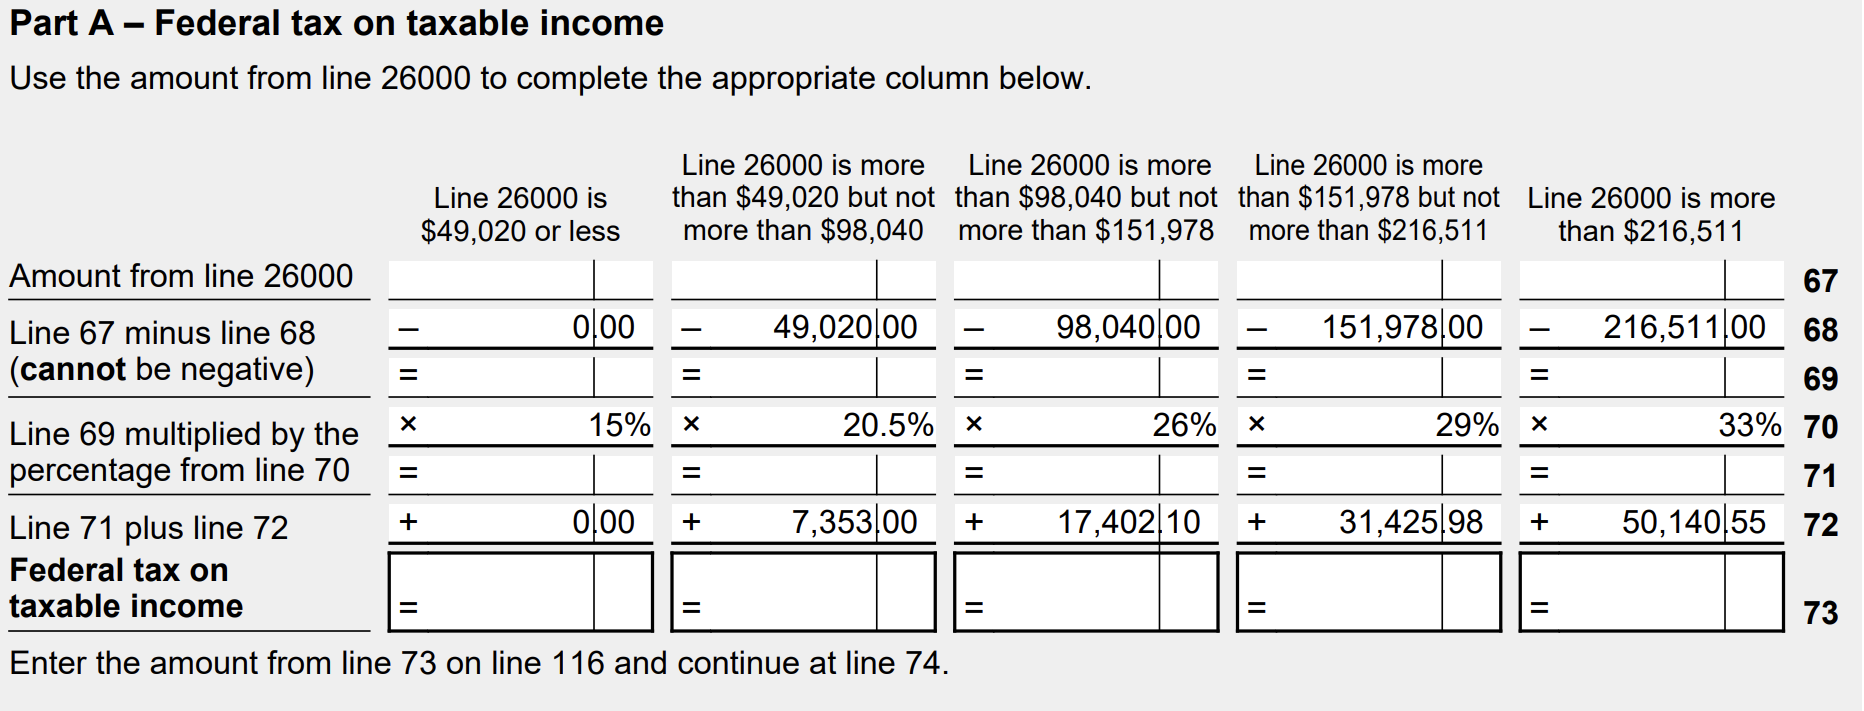
\includegraphics[width=0.6\linewidth]{Figures/Income_Tax}
		\end{figure}
		\begin{figure}
			\centering
			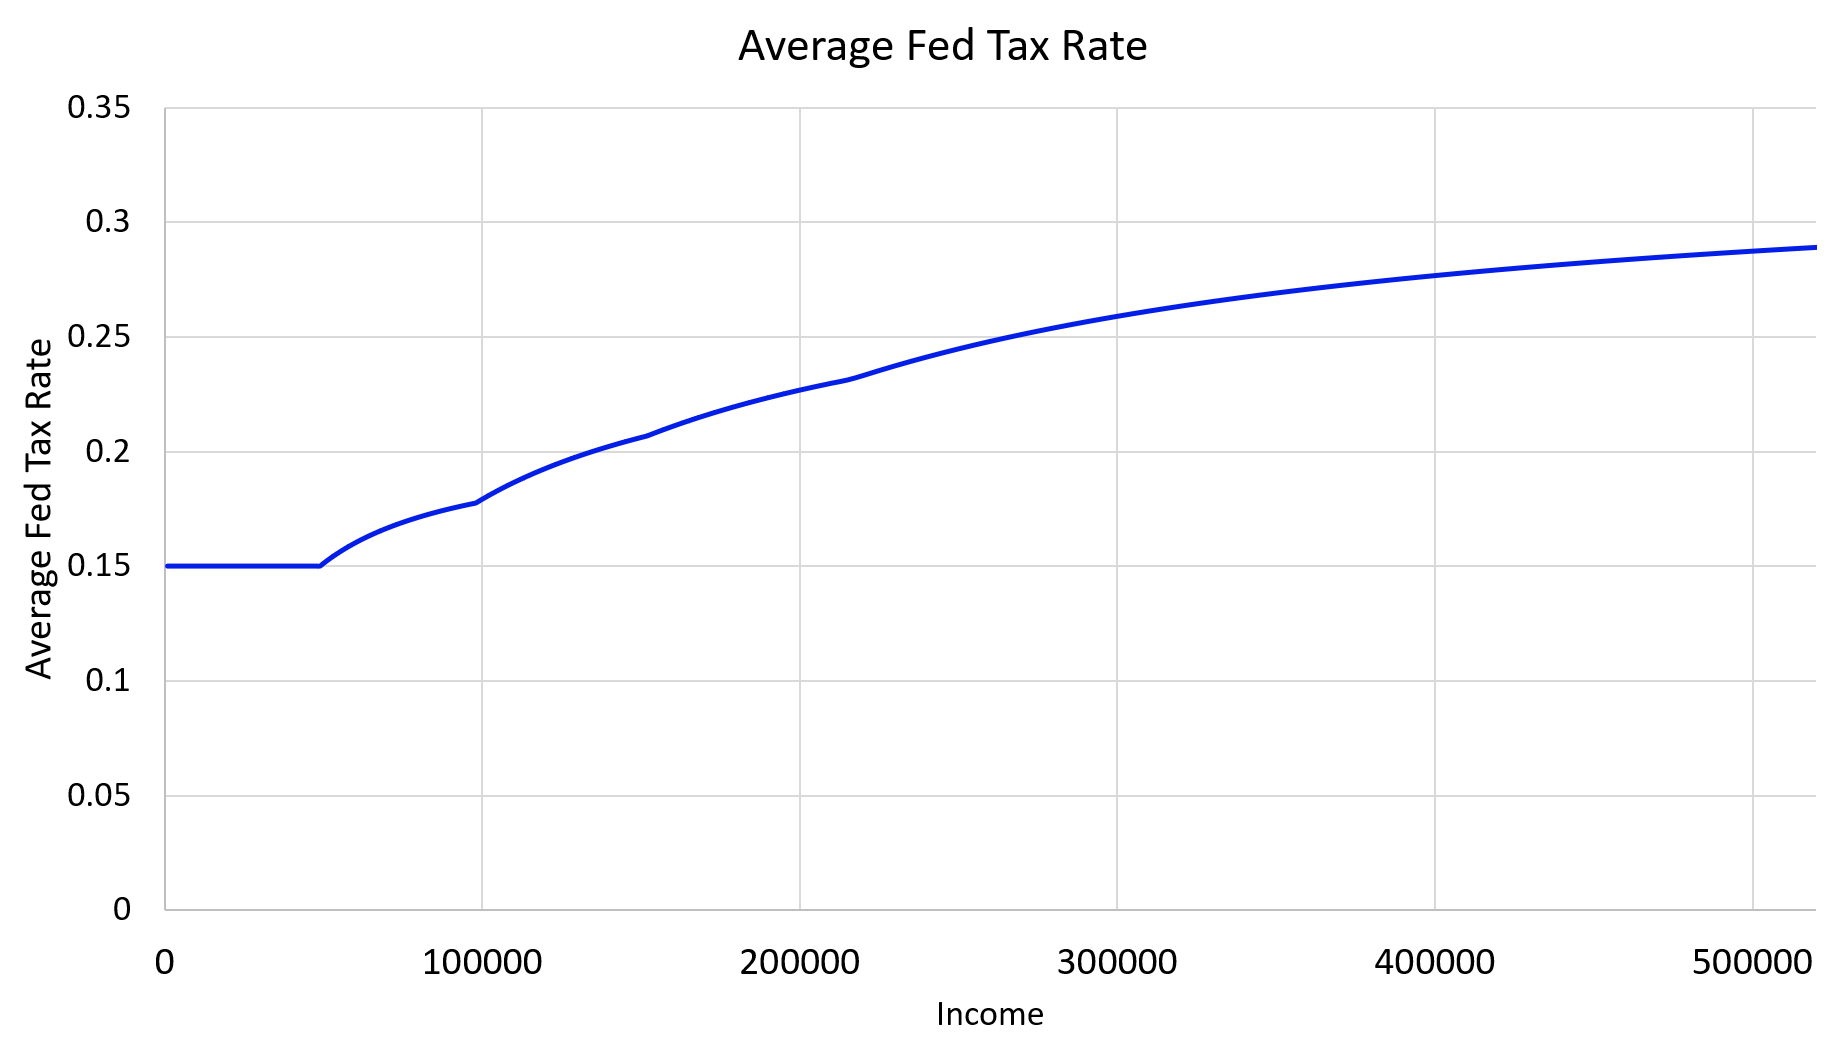
\includegraphics[width=0.55\linewidth]{Figures/average_fed_rate}
		\end{figure}
		
	\end{itemize}
\end{frame}

\begin{frame}[wide]{Fiscal Policy}
	\begin{itemize}
		\item The impact of fiscal policy depends on timing and the “no free lunch” principle
		\vspace{2mm}
		\item The problem of timing:
		\vspace{1mm}
		\begin{itemize}
			\item Discretionary changes often take a long time to implement. Tax credits, construction, education spending, and the like are put into place with delays
			\item Most discretionary fiscal policy require acknowledging a change in the economy, drafting legislation, passed by parliament, and approval by the executive branch
			\item Issues can arise and fiscal policy can have unintended effects if the shock that the legislation was designed to mitigate has passed
		\end{itemize}
	\end{itemize}
\end{frame}

\begin{frame}[wide]{Fiscal Policy}
	\begin{itemize}
		\item The “no free lunch” principle:
		\vspace{2mm}
		\begin{itemize}
			\item Government also faces a budget constraint
			\begin{itemize}
				\item Government spending + transfer payments=tax revenue
			\end{itemize}
			\item If it increases spending today, at some point in the future it must raise taxes or reduce spending
			\item Expecting the changes in the future, it may offset the stimulus today
		\end{itemize}
	\end{itemize}
\end{frame}

\begin{frame}[wide]{Ricardian Equivalence}
	\begin{itemize}
		\item According to Ricardian equivalence:
		\begin{itemize}
			\item The timing of tax changes does not matter for consumer behavior
			\begin{itemize}
				\item Permanent income hypothesis:	Consumption today is determined by the present discounted value of your lifetime income, after taxes
			\end{itemize}
			\item The present value of government tax collection determines behavior
		\end{itemize}
		\item Suppose government decides to increase government purchases by \$500 million
		\begin{figure}
			\centering
			\includegraphics[width=0.7\linewidth]{"Figures/fig 11_07"}
		\end{figure}
		\item The government spending leads to an increase in $\bar{a}_g$ (and $G$), but, given the expectation of an increase in future tax, the stimulus effect may be offset by the decrease in  consumption 
	\end{itemize}
\end{frame}

\begin{frame}[wide]{Net Exports}
	\begin{itemize}
		\item Trade balance = Net exports 
		\[EX-IM = \bar{a}_{ex}\bar{Y}_t -\bar{a}_{im}\bar{Y}_t = \left(\bar{a}_{ex} - \bar{a}_{im}\right)\bar{Y}_t\]
		\item When $EX>IM$, we have a trade surplus, $NX>0$
		\item When $EX<IM$, we have a trade deficit, $NX<0$
		\item Suppose there is an increase in demand for Canadian goods from Europe ($\bar{a}_{ex}$) $\implies$ IS shifts right $\implies$ an increase in short-run output
		\item Suppose there is an increase in Canadian's demand for Spanish wine ($\bar{a}_{im}$) $\implies$ IS shifts left $\implies$ a fall in short-run output
		
	\end{itemize}
\end{frame}

%\begin{frame}[wide]{An Increase in the Investment Rate}
%	\begin{columns} 
%			% Column 1
%			\begin{column}{.5\textwidth}
%				\begin{itemize}
%					\item Suppose the investment rate increases permanently for exogenous reasons ($s'>s$)
%					\begin{itemize}
%						\item The investment curve rotates upward ($\bar{s}'\bar{A}  \bar{L}^{1-\alpha} K_t^\alpha > \bar{s}\bar{A}  \bar{L}^{1-\alpha} K_t^\alpha$)
%						\item The depreciation curve remains unchanged ($\delta K_t$)
%						\item The capital stock increases by transition dynamics to reach the new steady state
%						\begin{itemize}
%							\item This happens because investment exceeds depreciation ($sY_t>\delta K_t$)
%						\end{itemize}
%						\item The new steady state is located to the right
%					\end{itemize}
%				\end{itemize}
%			\end{column}
%			% Column 2    
%			\begin{column}{.5\textwidth}			
%				\begin{figure}
%					\centering
%					\includegraphics[width=1\linewidth]{"Figures/An Increase in the Investment Rate"}
%				\end{figure}
%			\end{column}%
%		\end{columns}
%\end{frame}

%\begin{frame}[wide]{Measuring the State of the Economy}
%	\begin{columns} 
%		% Column 1
%		\begin{column}{.5\textwidth}
%			\begin{table}[htbp]
%				\centering
%				\begin{tabular}{lrrrr}
%					& 2005  & 2006  & 2007  & 2008 \\
%					\hline
%					GDP   & 12.6  & 13.4  & 14.0    & 14.3 \\
%					(in trillions of \$) &       &       &       &  \\
%					Growth rate GDP &       & 0.063 & 0.045 & 0.021 \\
%					\hline
%				\end{tabular}%
%				\label{tab:addlabel}%
%			\end{table}%
%		\end{column}
%		% Column 2    
%		\begin{column}{.5\textwidth}			
%			
%			
%		\end{column}%
%	\end{columns}
%\end{frame}

\begin{frame}[wide]{Next Lecture}
	\begin{itemize}
		\item Next lecture will begin Ch.12
	\end{itemize}
\end{frame}

\end{document}